\section{Web API}

\paragraph{Spørgsmål}
Redegør for og vis eksampler på hvordan man kan designe	og implementere et Web API inklusiv persistering af data i en database.	Og redegør for principperne i et RESTful Web API og	hvorledes man kan implementere et sådant.

\subsection{Web API}
Vi bruger et Web API for at lave en adskillelse af logik. Herved kan en applikations UI gøres udafhængig af den backend (forretningslogik).

\subsection{REST}
\textit{\textbf{RE}presentationnal \textbf{S}tate \textbf{T}ransfer} beskriver en række principper (ikke en standard) som web services kan designes efter. 

\begin{itemize}
	\item Brug HTTP verberne eksplicit.
	\item Vær stateless (og cacheable)
	\item Mappe-lignende URIs.
	\item Svare i JSON, XML eller lignede format.
\end{itemize}

\paragraph{Eksplicitte HTTP metoder}
Brug verberne eksplicit og kun til tiltænkte formål: 

\begin{multicols}{2}
\begin{itemize}
	\item GET
	\item POST
	\item PUT
	\item PATCH
	\item DELETE
	\item HEAD
\end{itemize}
\end{multicols}

\subsubsection{Cross-Origin Ressource Sharing}
Med CORS er det muligt at tillade andre servere at kald ens egen og på samme tid afvise andre. En ressource er på ''same origin'' hvis den har samme: scheme, host og port. Nedenstående figur viser forskellen.

\begin{figure}[h]
	\centering
	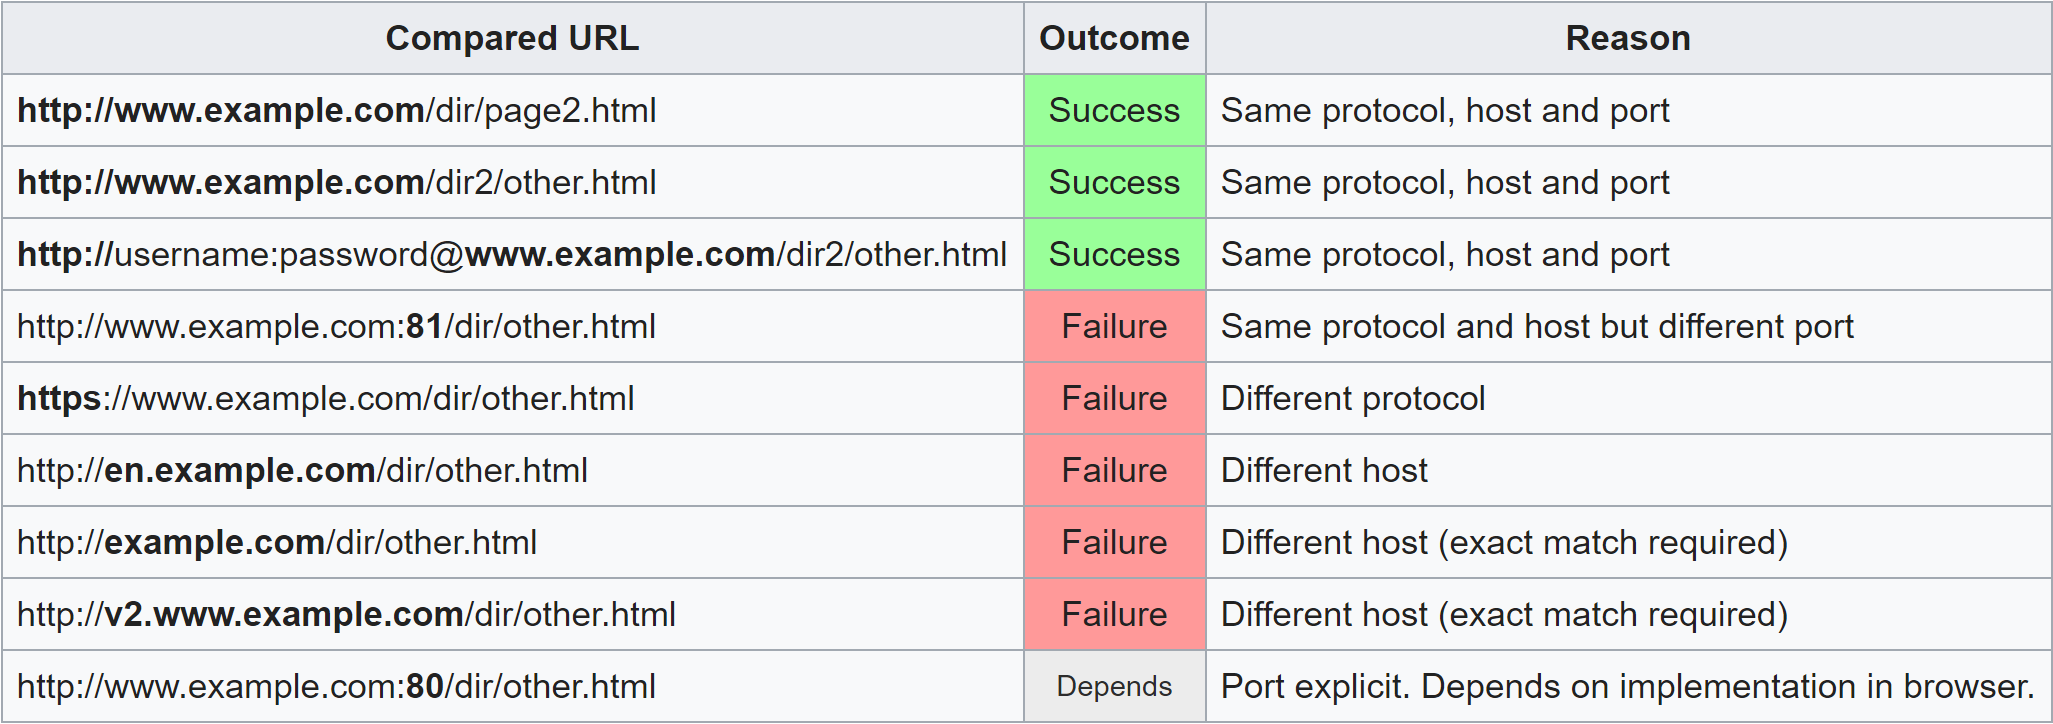
\includegraphics[width=\linewidth]{figs/spm6/cors-same-origin}
	\caption{Same origin defineret.}
	\label{fig:cors-same-origin}
\end{figure}
